\chapter{Implementierung}
\label{chapter:Implementierung}






%%%%%%%%%%%%%%%%%%%%%%%%%%%%%%%%%%%%%%%%%%%%%%%%%%%%%%%%%%%%%%%%%%%%%%%%%%%%%%%%%%%%
%%%%%%%%%%%%%%%%%%%%%%%%%%%%%%%%%%%%%%%%%%%%%%%%%%%%%%%%%%%%%%%%%%%%%%%%%%%%%%%%%%%%
%%%%%%%%%%%%%%%%%%%%%%%%%%%%%%%%%%%%%%%%%%%%%%%%%%%%%%%%%%%%%%%%%%%%%%%%%%%%%%%%%%%%
%%%%%%%%%%%%%%%%%%%%%%%%%%%%%%%%%%%%%%%%%%%%%%%%%%%%%%%%%%%%%%%%%%%%%%%%%%%%%%%%%%%%
%%%%%%%%%%%%%%%%%%%%%%%%%%%%%%%%%%%%%%%%%%%%%%%%%%%%%%%%%%%%%%%%%%%%%%%%%%%%%%%%%%%%
%%%%%%%%%%%%%%%%%%%%%%%%%%%%%%%%%%%%%%%%%%%%%%%%%%%%%%%%%%%%%%%%%%%%%%%%%%%%%%%%%%%%


\section{Schaltplan}
\label{section:Schaltplan}


\myboxy{
	\begin{itemize}
		\item Funktion (=Anlage) und Ortskennzeichen (+Ort) definieren. Funktionales Engineering.
		\item Bauteilkennzeichnung (BMK) festlegen.
		\item Aderfarben und Querschnitt definieren.
		\item Ausgewählte Bauteile in die Schaltung integrieren.
		\item Nicht vorhandene Bauteile selbst erstellen.
		      \begin{itemize}
			      \item Bauteile sortiert hinzufügen: Spannungsversorgung, Steuerung (Eingang, dann Ausgang), Lastkreis und Sonderfunktionen.
		      \end{itemize}
	\end{itemize}}{To-do}{\textwidth}



Zu Beginn der Erstellung des Schaltplans sollten die Funktions- und Ortskennzeichen sowie die Beschriftung der Bauteile und Leitungen festgelegt werden. Bei der Verdrahtung ist es erforderlich, die Aderfarben den entsprechenden Spannungspotenzialen zuzuordnen.

\subsection{Betriebsmittelbezeichnung}
\label{Schaltplan:BMK}

Ein Betriebsmittel besteht aus verschiedenen Kennzeichen: dem Funktionskennzeichen (=), dem Ortskennzeichen (+) und dem Betriebsmittelkennzeichen (-). Früher wurde das Funktionskennzeichen als „Anlage“ bezeichnet. In der neuen DIN EN IEC 81346-2 \cite{DIN_EN_IEC_81346-2} wurde diese Bezeichnung jedoch auf „Funktion“ geändert.

\subsubsection{Funktionskennzeichen}
Das Funktionskennzeichen beschreibt eine bestimmte Funktion im Schaltplan, wie beispielsweise die Spannungsversorgung oder die Steuerung (siehe Tabelle \ref{BMK:tab:funktionskennzeichen}).

\pagebreak[1]
\begin{table}[!ht]
	\centering
	\caption{Schaltplan – Funktionskennzeichen (=)}
	\label{BMK:tab:funktionskennzeichen}
	\begin{tabular}{ll}
		\hline
		\textbf{Abkürzung}      & \textbf{Bezeichnung} \\ \hline
		\multicolumn{1}{l|}{SV} & Spannungsversorung   \\
		\multicolumn{1}{l|}{ES} & Eingänge Steuerung   \\
		\multicolumn{1}{l|}{AS} & Ausgänge Steuerung   \\
		\multicolumn{1}{l|}{KO} & Kommunikation        \\
		\multicolumn{1}{l|}{AT} & Antrieb              \\
		\multicolumn{1}{l|}{NA} & Not-Aus              \\ \hline
	\end{tabular}
\end{table}
\pagebreak[1]

\subsubsection{Ortskennzeichen}
Das Ortskennzeichen gibt an, an welchem Ort ein Bauteil installiert ist. Beispielsweise gibt es im Fahrzeug eine Steuereinheit und eine Batterieeinheit. Im Schaltplan wird dadurch deutlich, welche Verbindungen zwischen verschiedenen Orten bestehen. Das Ortskennzeichen erleichtert zudem die Wartung und Installation des Systems.

\pagebreak[1]
\begin{table}[!ht]
	\centering
	\caption{Schaltplan – Ortskennzeichen (+)}
	\label{bmk:tab:ortskennzeichen}
	\begin{tabular}{ll}
		\hline
		\textbf{Abkürzung}       & \textbf{Bezeichnung} \\ \hline
		\multicolumn{1}{l|}{POD} & Fahrzeug             \\
		\multicolumn{1}{l|}{BE}  & Batterieeinheit      \\
		\multicolumn{1}{l|}{SE}  & Steuereinheit        \\
		\multicolumn{1}{l|}{AE}  & Antriebseinheit      \\ \hline
	\end{tabular}
\end{table}
\pagebreak[1]

\subsubsection{Betriebsmittelkennzeichen}
Das Betriebsmittelkennzeichen bezeichnet das spezifische Bauteil. Die genaue Zuordnung der Bezeichnungen ist in der DIN EN IEC 81346-2 geregelt. Die für das Projekt relevanten Betriebsmittelkennzeichen sind in Tabelle \ref{bmk:tab:betriebsmittelkennzeichen} aufgeführt.



\pagebreak[1]
\begin{table}[!ht]
	\centering
	\caption{Schaltplan – Betriebsmittelkennzeichen (-) \cite{DIN_EN_IEC_81346-2}}
	\label{bmk:tab:betriebsmittelkennzeichen}
	\begin{tabular}{|l|lll|}
		\hline
		\textbf{Abkürzung}       & \textbf{Klassenname}                            & \multicolumn{1}{l|}{\textbf{Allgemeine Bedeutung}} \\ \hline
		\multicolumn{1}{|l|}{FC} & \makecell[l]{Überstromschutzobjekt}             & \multicolumn{1}{l|}{Sicherung}                     \\ \hline
		\multicolumn{1}{|l|}{GB} & \makecell[l]{Erzeugungsobjekt für elektrische                                                        \\Energie durch chemische Energie} & \multicolumn{1}{l|}{Batterie} \\ \hline
		\multicolumn{1}{|l|}{KE} & \makecell[l]{Elektrische Signale                                                                     \\verarbeitendes Objekt}   & \multicolumn{1}{l|}{Steuerung} \\ \hline
		\multicolumn{1}{|l|}{MA} & \makecell[l]{Elektromagnetisches                                                                     \\Rotationsantriebsobjekt} & \multicolumn{1}{l|}{Motor} \\ \hline
		\multicolumn{1}{|l|}{QA} & \makecell[l]{Stromsteuerungsobjekt}             & \multicolumn{1}{l|}{Relais}                        \\ \hline
		\multicolumn{1}{|l|}{RL} & \makecell[l]{Bewegungsbegrenzungsobjekt}        & \multicolumn{1}{l|}{Bremse}                        \\ \hline
		\multicolumn{1}{|l|}{SF} & \makecell[l]{Gesichtsinteraktionsobjekt}        & \multicolumn{1}{l|}{Schalter}                      \\ \hline
		\multicolumn{1}{|l|}{TB} & \makecell[l]{Stromkonvertierungsobjekt}         & \multicolumn{1}{l|}{Transformator}                 \\ \hline
		\multicolumn{1}{|l|}{WD} & \makecell[l]{Niederspannungsenergie Leitobjekt} & \multicolumn{1}{l|}{Leitung/Kabel}                 \\ \hline
		\multicolumn{1}{|l|}{XD} & \makecell[l]{Niederspannungs-Verbindungsobjekt} & \multicolumn{1}{l|}{Klemme, Stecker oder Buchse}   \\ \hline
	\end{tabular}
\end{table}
\pagebreak[1]

Bei einer vollständigen Betriebsmittelbezeichnung sieht das Kennzeichen des Betriebsmittels folgendermaßen aus:

\begin{center} =ES2+SE1-10QA1 \end{center}

Die Betriebsmittelbezeichnung =ES2+SE1-10QA4 besagt, dass es sich um die Eingänge der Steuerung (=ES) handelt. Hierbei gibt es zwei Funktionen. Der Ort ist in der Steuereinheit (+SE) verortet, und das Betriebsmittel selbst ist ein Relais, welche auf der Seite 10 des Schaltplans zu finden ist.

Das Kennzeichen umfasst sowohl das Funktions- als auch das Ortskennzeichen, die jeweils mit einer fortlaufenden Nummer versehen sind. Das Betriebsmittelkennzeichen enthält zwei Nummerierungen: Die erste gibt an, auf welcher Seite des Schaltplans sich das Betriebsmittel befindet, während die zweite die fortlaufende Nummerierung des Bauteils darstellt.\\
Im Schaltplan wird das Betriebsmittel lediglich durch das Betriebsmittelkennzeichen (-) dargestellt, während das Funktions- und Ortskennzeichen im Zeichnungskopf angegeben ist.

\newpage

\subsection{Verdrahtung Konventionen}
\label{section:Verdrahtung_Konventionen}
Für die Verdrahtung müssen den Spannungspotenzialen verschiedene Farben zugewiesen werden. Diese Zuordnungen sind in Tabelle \ref{Verdrahtung_Konventionen:tab:Zuordnung} aufgeführt.
\pagebreak[1]
\begin{table}[!ht]
	\centering
	\caption{Verdrahtung Konvention – Aderfarben}
	\label{Verdrahtung_Konventionen:tab:Zuordnung}
	\begin{tabular}{llccl}
		\hline
		\textbf{Name} & \textbf{Fabe}                 & \textbf{U in V} & \textbf{A in mm$^2$} & \textbf{Funktion} \\ \hline
		              & \multicolumn{1}{l|}{Rot}      & $x$             & 1                    &                   \\
		              & \multicolumn{1}{l|}{Blau}     & $x$             & 1                    &                   \\
		              & \multicolumn{1}{l|}{Schwarz}  & $x$             & 1                    &                   \\
		              & \multicolumn{1}{l|}{Schwarz}  & $< 48$          & 50                   &                   \\
		              & \multicolumn{1}{l|}{Viollett} & $x$             & 1                    &                   \\ \hline
	\end{tabular}
\end{table}
\pagebreak[4]




%%%%%%%%%%%%%%%%%%%%%%%%%%%%%%%%%%%%%%%%%%%%%%%%%%%%%%%%%%%%%%%%%%%%%%%%%%%%%%%%%%%%
%%%%%%%%%%%%%%%%%%%%%%%%%%%%%%%%%%%%%%%%%%%%%%%%%%%%%%%%%%%%%%%%%%%%%%%%%%%%%%%%%%%%
%%%%%%%%%%%%%%%%%%%%%%%%%%%%%%%%%%%%%%%%%%%%%%%%%%%%%%%%%%%%%%%%%%%%%%%%%%%%%%%%%%%%
%%%%%%%%%%%%%%%%%%%%%%%%%%%%%%%%%%%%%%%%%%%%%%%%%%%%%%%%%%%%%%%%%%%%%%%%%%%%%%%%%%%%
%%%%%%%%%%%%%%%%%%%%%%%%%%%%%%%%%%%%%%%%%%%%%%%%%%%%%%%%%%%%%%%%%%%%%%%%%%%%%%%%%%%%
%%%%%%%%%%%%%%%%%%%%%%%%%%%%%%%%%%%%%%%%%%%%%%%%%%%%%%%%%%%%%%%%%%%%%%%%%%%%%%%%%%%%

\newpage
\section{Simulation mit Simulink}
\label{section:Simulation}

\myboxy{
	\begin{itemize}
		\item
	\end{itemize}
}{To-do}{\textwidth}


\subsection{Funktionsweise der Steuerung}
\label{Steuerung}

%Das Fahrzeug wird mittels eines Moore-Automaten gesteuert, wie in Abbildung \ref{Automat:img:Automat} dargestellt. Die Zustände $\overrightarrow{Z}$ (siehe Gleichung \ref{Automat:equation:vektor_z_auto}), die Eingänge $\overrightarrow{I}$ (siehe Gleichung \ref{Automat:equation:vektor_i}) und die Ausgänge $\overrightarrow{O}$ (siehe Gleichung \ref{Automat:equation:vektor_o}) können in Vektoren dargestellt werden.\\ \ \\

Die Steuerung des Fahrzeugs bietet die Möglichkeit, zwischen Automatik- und manuellem Betrieb zu wählen. Im manuellen Betrieb kann der Benutzer das Fahrzeug sowohl vorwärts als auch rückwärts fahren lassen, wobei zwei Geschwindigkeitsstufen – schnell und langsam – zur Verfügung stehen. Diese Funktion soll die möglichkeit geben666\\
Der Automatikmodus wird über den Startknopf aktiviert. Das Fahrzeug beschleunigt auf die einstellbare Geschwindigkeit und bremst automatisch ab, sobald die Distanz zum Enddeckel der Röhre kleiner wird. Es hält schließlich am Ende der Strecke an.\\

\subsubsection{Controllpanel}
\label{Steuerung:Controllpanel}
Über das Control Panel (siehe Abbildung \ref{Controllpanel:img:Controllpanel}) können alle Eingaben via Simulink gesteuert werden. Mit dem Wahlschalter kann, wie bereits erwähnt, zwischen Automatik- und manuellem Betrieb gewechselt werden. Ist der manuelle Betrieb ausgewählt, kann mit dem Drehschalter (Manuell) zwischen Vorwärts, Rückwärts und Stopp geschaltet werden (siehe Tabelle \ref{Controllpanel:tab:Wahlschalter}, die Werte werden später für die Automatensteuerung benötigt).\\


\pagebreak[1]
\begin{table}[!ht]
	\centering
	\caption{Automat – Wahlschalter für den manuellen Betrieb}
	\label{Controllpanel:tab:Wahlschalter}
	\begin{tabular}{ccc}
		\hline
		\textbf{Schalterbezeichnung} & \textbf{Zustände} & \textbf{Wert} \\ \hline
		\multicolumn{1}{c|}{Rück+}   & Forwards fast     & 1             \\
		\multicolumn{1}{c|}{Rück}    & Forwards slow     & 2             \\
		\multicolumn{1}{c|}{STOP}    & Manual idle       & 3             \\
		\multicolumn{1}{c|}{Vor}     & Backwards slow    & 4             \\
		\multicolumn{1}{c|}{Vor+}    & Backwards fast    & 5             \\ \hline
	\end{tabular}
\end{table}
\pagebreak[3]
Im Automatikbetrieb kann die Geschwindigkeit über das Drehrad \frqq Geschwindigkeit Automatik\flqq\ voreingestellt oder während der Fahrt angepasst werden. Das Fahrzeug beginnt zu fahren, sobald der Druckknopf \frqq Start\flqq\ betätigt wird. Die Automatik kann über den Druckknopf \frqq Stop\flqq\ gestoppt werden.\\ Im Notfall kann sowohl im Automatik- als auch im manuellen Betrieb der Druckknopf \frqq Emergency stop\flqq\ betätigt werden. Das Fahrzeug führt eine Vollbremsung mit der Motor- und der mechanischen Bremse durch. Der Notfallmodus kann durch Drücken des \frqq Reset\flqq\ -Knopfs beendet werden.\\
Die Funktionsweise der manuellen Steuerung wird in Abschnitt \ref{Automatensteuerung:Automat_man} erklärt, und die der automatischen Steuerung in Abschnitt \ref{Automatensteuerung:Automat_auto}


\pagebreak[1]
\begin{figure}[!ht]
	\begin{center}
		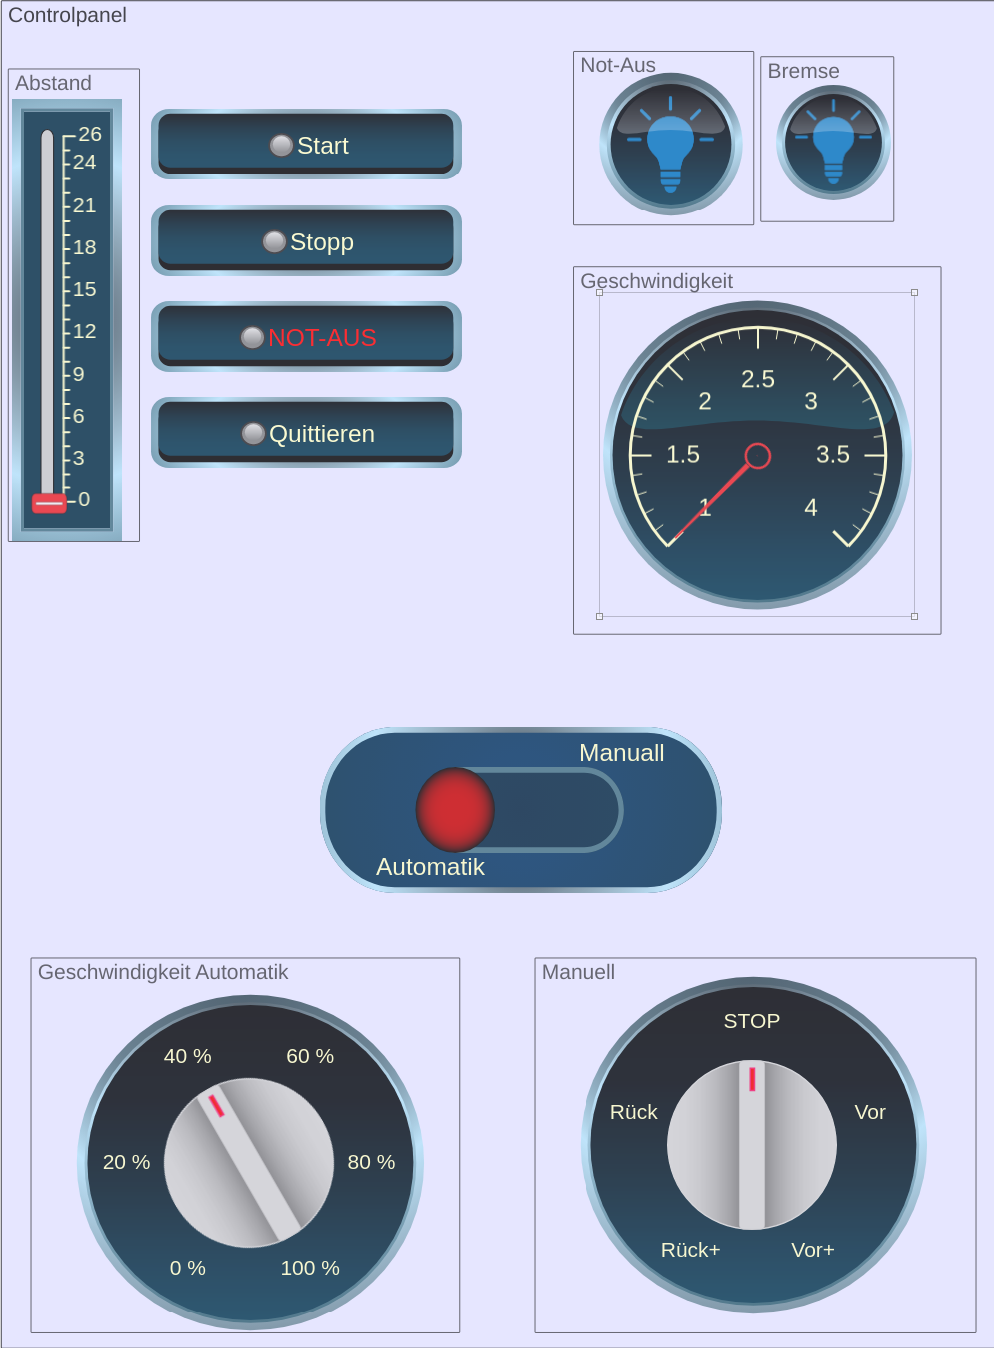
\includegraphics[width=0.75\textwidth]{img/5_simulation/Automat_con.png}
		\caption{Automat – Controllpanel}
		\label{Controllpanel:img:Controllpanel}
	\end{center}
\end{figure}
\pagebreak[4]


\subsection{Automatensteuerung}
\label{Automatensteuerung}
Die Automatensteuerung beschreibt die logische Steuerung eines Systems durch einen Automaten, wie etwa einen Moore- oder Mealy-Automaten, der auf Basis von Eingaben und aktuellen Zuständen Ausgaben steuert.\\
Das Fahrzeug wird mittels eines Moore-Automaten gesteuert, wobei die Ausgänge erst dann aktiviert werden, wenn sich das System im entsprechenden Zustand befindet.\\ \ \\
Der Automat startet im Zustand \frqq Idle\flqq siehe Abbildung \ref{Automat_man:tab:z_idle}, und die Abläufe für den automatischen oder manuellen Modus werden von \frqq Idle\flqq\ aus angesteuert. Im Zustand Idle werden die Ausgänge (siehe Tabelle \ref{Automat_man:tab:z_idle}) geschaltet.\\

\pagebreak[1]
\begin{figure}[!ht]
	\begin{center}
		\includegraphics[width=0.75\textwidth]{img/5_simulation/Automat_idle.png}
		\caption{Automat – Start Zustand \frqq Idle\flqq}
		\label{Automat_man:img:start_idle}
	\end{center}
\end{figure}
\pagebreak[4]


\pagebreak[1]
\begin{table}[!ht]
	\centering
	\caption{Ausgänge – Idle}
	\label{Automat_man:tab:z_idle}
	\begin{tabular}{lll}
		\hline
		\textbf{Ausgänge}                           & \textbf{I/O Module}                 & \textbf{Wert} \\ \hline
		\multicolumn{1}{l|}{speed out}              & \multicolumn{1}{l|}{IO397-50k – A1} & 1             \\
		\multicolumn{1}{l|}{Driving(1)}             & \multicolumn{1}{l|}{}               & Reset         \\
		\multicolumn{1}{l|}{break motor out}        & \multicolumn{1}{l|}{IO397-50k – B3} & 5             \\
		\multicolumn{1}{l|}{direction out}          & \multicolumn{1}{l|}{IO397-50k – B4} & 5             \\
		\multicolumn{1}{l|}{cruise out}             & \multicolumn{1}{l|}{IO397-50k – B5} & 5             \\
		\multicolumn{1}{l|}{break mechanically out} & \multicolumn{1}{l|}{IO397-50k – B6} & 5             \\
		\multicolumn{1}{l|}{emergency stop out}     & \multicolumn{1}{l|}{IO397-50k – B7} & 0             \\ \hline
	\end{tabular}
\end{table}
\pagebreak[1]

Die Funktion \frqq Driving\flqq, siehe Abbildung \ref{Automat:img:fnc_Driving}, erhält einen Eingangswert, der durch einen \frqq Rate Limiter\flqq\ begrenzt und am Ausgang ausgegeben wird. Die Funktion speichert den letzten Wert, daher muss sie in den Zuständen, in denen das Fahrzeug angehalten wird, zurückgesetzt werden. Dies geschieht, indem die Funktion \frqq Driving\flqq\ den Wert \frqq 1\flqq\ erhält.\\

\pagebreak[1]
\begin{figure}[!ht]
	\begin{center}
		\includegraphics[width=.5\textwidth]{img/5_simulation/Automat_funktion_1.png}
		\includegraphics[width=.75\textwidth]{img/5_simulation/Automat_funktion_2.png}
		\caption{Automat – Funktion Driving}
		\label{Automat:img:fnc_Driving}
	\end{center}
\end{figure}
\pagebreak[4]

Der Zustand \frqq Emergency stop\flqq\ kann von jedem Zustand aus durch den Eingang \frqq emergency stop in\flqq\ erreicht werden, welcher sowohl über das Controllpanel als auch extern über das IO397-50k – B11 ausgelöst werden kann. Der Zustand kann nur durch ein Reset-Signal verlassen werden und führt dann in einen der Idle-Zustände zurück: \frqq Idle\flqq\ \frqq Manual idle\flqq\ oder \frqq Automatic idle\flqq. Im Zustand \frqq Emergency stop\flqq\ werden die Ausgänge gemäß Tabelle \ref{Automat_man:tab:z_Emergency_stop} geschaltet.


\pagebreak[1]
\begin{table}[!ht]
	\centering
	\caption{Ausgänge – Emergency stop}
	\label{Automat_man:tab:z_Emergency_stop}
	\begin{tabular}{lll}
		\hline
		\textbf{Ausgänge}                           & \makecell{\textbf{I/O Module}         \\ \textbf{IO397-50k}}                 & \textbf{Wert} \\ \hline
		\multicolumn{1}{l|}{speed out=Driving()}    & \multicolumn{1}{l|}{A1}       & Reset \\
		\multicolumn{1}{l|}{break motor out}        & \multicolumn{1}{l|}{}         & 5     \\
		\multicolumn{1}{l|}{direction out}          & \multicolumn{1}{l|}{B4}       & 5     \\
		\multicolumn{1}{l|}{cruise out}             & \multicolumn{1}{l|}{B5}       & 5     \\
		\multicolumn{1}{l|}{break mechanically out} & \multicolumn{1}{l|}{B6}       & 5     \\
		\multicolumn{1}{l|}{emergency stop out}     & \multicolumn{1}{l|}{B7}       & 5     \\ \hline
	\end{tabular}
\end{table}
\pagebreak[1]










\subsubsection{Automat für die manuelle Steuerung}
\label{Automatensteuerung:Automat_man}

Die manuelle Steuerung bietet dem Nutzer die Flexibilität, das Fahrzeug sowohl innerhalb als auch außerhalb der Röhre zu steuern.\\

Der Automat des manuellen Ablaufs, wie in Abbildung \ref{Automat_man:img:man_übersicht} dargestellt, ist in zwei Stateflows unterteilt: \frqq Forwards\flqq\ und \frqq Backwards\flqq . In Abbildung \ref{Automat_man:img:man_vorwärts} ist der \frqq Forwards\flqq\ -Stateflow zu sehen, der \frqq Backwards\flqq\ -Stateflow ist äquivalent, wobei sich lediglich der Ausgang \frqq Direction Out\flqq\ ändert. Daher wird nur der \frqq Forwards\flqq\ -Stateflow erklärt. Der Zustand \frqq Emerency stop 1\flqq\ ist der gleiche Zustand wie \frqq Emerency stop\flqq. Die Ausgänge für die Zustände \frqq Forwards\flqq\ und \frqq Backwards\flqq\ sind in der Tabelle \ref{Automat_man:tab:z_V_langsam} für die Zustände \frqq slow\flqq\ und in der Tabelle \ref{Automat_man:tab:z_V_schnell} für die Zustände \frqq fast\flqq\ aufgelistet.




\pagebreak[1]
\begin{figure}[!ht]
	\begin{center}
		\includegraphics[width=0.9\textwidth]{img/5_simulation/Automat_man_uebersicht.png}
		\caption{Automat – Übersicht der manuellen Steuerung}
		\label{Automat_man:img:man_übersicht}
	\end{center}
\end{figure}
\pagebreak[1]


\pagebreak[1]
\begin{table}[!ht]
	\centering
	\caption{Ausgänge – der Zustände \frqq Forwards\flqq\ und \frqq Backwards\flqq\ –  \frqq slow\flqq}
	\label{Automat_man:tab:z_V_langsam}
	\begin{tabular}{llcc}
		\hline
		\textbf{Ausgänge}                             & \makecell{\textbf{I/O Module}             \\ \textbf{IO397-50k}}     & \makecell{\textbf{Werte}       \\ \textbf{\frqq Forwards\flqq}} & \makecell{\textbf{Werte}     \\ \textbf{\frqq Backwards\flqq}}  \\ \hline
		\multicolumn{1}{l|}{speed out=Driving$(1,5)$} & \multicolumn{1}{l|}{A1}       & 1,5 & 1,5 \\
		\multicolumn{1}{l|}{break motor out}          & \multicolumn{1}{l|}{B3}       & 1   & 1   \\
		\multicolumn{1}{l|}{direction out}            & \multicolumn{1}{l|}{B4}       & 5   & 0   \\
		\multicolumn{1}{l|}{cruise out}               & \multicolumn{1}{l|}{B5}       & 5   & 5   \\
		\multicolumn{1}{l|}{break mechanically out}   & \multicolumn{1}{l|}{B6}       & 0   & 0   \\
		\multicolumn{1}{l|}{emergency stop out}       & \multicolumn{1}{l|}{B7}       & 0   & 0   \\ \hline
	\end{tabular}
\end{table}
\pagebreak[1]

\pagebreak[1]
\begin{table}[!ht]
	\centering
	\caption{Ausgänge – der Zustände \frqq Forwards\flqq\ und \frqq Backwards\flqq\ –  \frqq fast\flqq}
	\label{Automat_man:tab:z_V_schnell}
	\begin{tabular}{cccc}
		\hline
		\textbf{Ausgänge}                           & \makecell{\textbf{I/O Module}         \\ \textbf{IO397-50k}}    & \makecell{\textbf{Werte}     \\ \textbf{\frqq Forwards\flqq}} & \makecell{\textbf{Werte}     \\ \textbf{\frqq Backwards\flqq}} \\ \hline
		\multicolumn{1}{l|}{speed out=Driving$(3)$} & \multicolumn{1}{l|}{A1}       & 3 & 3 \\
		\multicolumn{1}{l|}{break motor out}        & \multicolumn{1}{l|}{B3}       & 1 & 1 \\
		\multicolumn{1}{l|}{direction out}          & \multicolumn{1}{l|}{B4}       & 5 & 0 \\
		\multicolumn{1}{l|}{cruise out}             & \multicolumn{1}{l|}{B5}       & 5 & 5 \\
		\multicolumn{1}{l|}{break mechanically out} & \multicolumn{1}{l|}{B6}       & 0 & 0 \\
		\multicolumn{1}{l|}{emergency stop out}     & \multicolumn{1}{l|}{B7}       & 0 & 0 \\ \hline
	\end{tabular}
\end{table}
\pagebreak[1]

\pagebreak[1]
\begin{figure}[!ht]
	\begin{center}
		\includegraphics[width=\textwidth]{img/5_simulation/Automat_man_vorwaerts.png}
		\caption{Automat – \frqq Forwards\flqq\ -Stateflow der manuellen Steuerung}
		\label{Automat_man:img:man_vorwärts}
	\end{center}
\end{figure}
\pagebreak[1]



Mit dem Wahltaster (siehe Tabelle \ref{Controllpanel:tab:Wahlschalter}) kann zwischen den Zuständen gewechselt werden. In der Abbildung \ref{Automat_man:img:man_vorwärts} ist der Ausschnitt des \frqq Forwards\flqq\ -Stateflow zu sehen. Wenn sich der Automat in dem Stateflow \frqq Forwards\flqq\ befindet, gibt es keine direkte verknüpfung zu dem \frqq Backwards\flqq\ Stateflow, somit muss man erst in den Zustand \frqq Manual idle\flqq\ wechseln, um in den Stateflow \frqq Backwards\flqq\ zu gelangen.

Der Zustand \frqq Collector manual in\flqq\ fängt  das Schaltsignal des Wahlschalters ab, wenn mitten im Betrieb auf Automatik geschalten wird und führt zu dem \frqq Idle \flqq\ Zustand.









\subsubsection{Automat für die automatische Steuerung}
\label{Automatensteuerung:Automat_auto}


Die automatische Steuerung soll das Fahrzeug innerhalb der Röhre bis zur eingestellten Geschwindigkeit beschleunigen. Ab einer bestimmten Distanz zum Ende der Röhre soll es allmählich abbremsen und schließlich zum Stillstand kommen.

Der Automat \frqq Automatic\flqq\ besteht aus den Zuständen \frqq Automatic\flqq, \frqq Drive\flqq, \frqq Distance\flqq, \frqq Stop\flqq\ und \frqq Emergency stop\flqq, die in Abbildung \ref{Automat:img:auto_übersicht} dargestellt sind.\\
Der Zustand \frqq Automatic\flqq\ beschreibt den Idle-Zustand der automatischen Steuerung. Von hier aus wird der Zustand \frqq Drive\flqq\ angesteuert, sobald der Startknopf des \frqq Control Panels\flqq\ (siehe Abbildung \ref{Controllpanel:img:Controllpanel}) betätigt wird. Die Ausgänge werden gemäß Tabelle \ref{Automat_man:tab:automatic} gesetzt, solange der Zustand \frqq Automatic\flqq\ nicht verlassen wird.\\
Im Zustand \frqq Drive\flqq\ wird die Geschwindigkeit vom Nutzer mittels des Drehrads \frqq Geschwindigkeit Automatik\flqq\ eingestellt. Wird hingegen der \frqq Stop\flqq\ Taster betätigt, wird der Zustand \frqq Stop\flqq\ angesteuert. Ab einer Distanz von 10 m wird der Zustand \frqq Distance\flqq\ aktiviert. In Tabelle \ref{Automat_man:tab:drive} sind die Ausgänge des Zustands \frqq Drive\flqq\ dargestellt.\\
Wie bereits erwähnt, wird die Geschwindigkeit in Abhängigkeit zum Abstand \frqq distance\flqq\ vom Ende der Röhre verringert, hier bei wird in dem Zustand \frqq Distance\flqq\ der Augang der Geschwindigkeit mittels der Gleichung:

\pagebreak[1]
\begin{align}
	\label{eq:speedout}
	speed_{out} = distance_{in}\cdot\frac{speed_{in}-1}{distance}+1
\end{align}
\pagebreak[1]

ermittelt.

Soll die Automatik beendet werden, kann dies über den Stop-Taster auf dem Control Panel ausgelöst werden. Dabei werden die in Tabelle \ref{Automat_man:tab:stop} aufgeführten Signale geschaltet.

\pagebreak[1]
\begin{table}[!ht]
	\centering
	\caption{Ausgänge – Automatic}
	\label{Automat_man:tab:automatic}
	\begin{tabular}{lll}
		\hline
		\textbf{Ausgänge}                           & \makecell{\textbf{I/O Module}             \\ \textbf{IO397-50k}}                 & \textbf{Wert} \\ \hline
		\multicolumn{1}{l|}{speed out}              & \multicolumn{1}{l|}{A1}       & Driving() \\
		\multicolumn{1}{l|}{Driving(1)}             & \multicolumn{1}{l|}{}         & Reset     \\
		\multicolumn{1}{l|}{break motor out}        & \multicolumn{1}{l|}{B3}       & 5         \\
		\multicolumn{1}{l|}{direction out}          & \multicolumn{1}{l|}{B4}       & 5         \\
		\multicolumn{1}{l|}{cruise out}             & \multicolumn{1}{l|}{B5}       & 5         \\
		\multicolumn{1}{l|}{break mechanically out} & \multicolumn{1}{l|}{B6}       & 5         \\
		\multicolumn{1}{l|}{emergency stop out}     & \multicolumn{1}{l|}{B7}       & 5         \\ \hline
	\end{tabular}
\end{table}
\pagebreak[2]



\pagebreak[1]
\begin{table}[!ht]
	\centering
	\caption{Ausgänge – Drive}
	\label{Automat_man:tab:drive}
	\begin{tabular}{lll}
		\hline
		\textbf{Ausgänge}                           & \makecell{\textbf{I/O Module}                     \\ \textbf{IO397-50k}}                 & \textbf{Wert} \\ \hline
		\multicolumn{1}{l|}{speed out}              & \multicolumn{1}{l|}{A1}       & Driving(speed in) \\
		\multicolumn{1}{l|}{Driving(speed in)}      & \multicolumn{1}{l|}{}         & speed in          \\
		\multicolumn{1}{l|}{break motor out}        & \multicolumn{1}{l|}{B3}       & 5                 \\
		\multicolumn{1}{l|}{direction out}          & \multicolumn{1}{l|}{B4}       & 5                 \\
		\multicolumn{1}{l|}{cruise out}             & \multicolumn{1}{l|}{B5}       & 5                 \\
		\multicolumn{1}{l|}{break mechanically out} & \multicolumn{1}{l|}{B6}       & 5                 \\
		\multicolumn{1}{l|}{emergency stop out}     & \multicolumn{1}{l|}{B7}       & 5                 \\ \hline
	\end{tabular}
\end{table}
\pagebreak[2]


\pagebreak[1]
\begin{table}[!ht]
	\centering
	\caption{Ausgänge – Distance}
	\label{Automat_man:tab:distance}
	\begin{tabular}{lll}
		\hline
		\textbf{Ausgänge}                           & \makecell{\textbf{I/O Module}                         \\ \textbf{IO397-50k}}                 & \textbf{Wert} \\ \hline
		\multicolumn{1}{l|}{speed out}              & \multicolumn{1}{l|}{A1}       & gl. \ref{eq:speedout} \\
		\multicolumn{1}{l|}{Driving(1)}             & \multicolumn{1}{l|}{}         & distance in           \\
		\multicolumn{1}{l|}{break motor out}        & \multicolumn{1}{l|}{B3}       & 1                     \\
		\multicolumn{1}{l|}{direction out}          & \multicolumn{1}{l|}{B4}       & 5                     \\
		\multicolumn{1}{l|}{cruise out}             & \multicolumn{1}{l|}{B5}       & 5                     \\
		\multicolumn{1}{l|}{break mechanically out} & \multicolumn{1}{l|}{B6}       & 0                     \\
		\multicolumn{1}{l|}{emergency stop out}     & \multicolumn{1}{l|}{B7}       & 0                     \\ \hline
	\end{tabular}
\end{table}
\pagebreak[2]


\pagebreak[1]
\begin{table}[!ht]
	\centering
	\caption{Ausgänge – Stop}
	\label{Automat_man:tab:stop}
	\begin{tabular}{lll}
		\hline
		\textbf{Ausgänge}                           & \makecell{\textbf{I/O Module}             \\ \textbf{IO397-50k}}                 & \textbf{Wert} \\ \hline
		\multicolumn{1}{l|}{speed out}              & \multicolumn{1}{l|}{A1}       & Driving() \\
		\multicolumn{1}{l|}{Driving(Reset)}         & \multicolumn{1}{l|}{}         & Reset     \\
		\multicolumn{1}{l|}{break motor out}        & \multicolumn{1}{l|}{B3}       & 1         \\
		\multicolumn{1}{l|}{direction out}          & \multicolumn{1}{l|}{B4}       & 5         \\
		\multicolumn{1}{l|}{cruise out}             & \multicolumn{1}{l|}{B5}       & 5         \\
		\multicolumn{1}{l|}{break mechanically out} & \multicolumn{1}{l|}{B6}       & 0         \\
		\multicolumn{1}{l|}{emergency stop out}     & \multicolumn{1}{l|}{B7}       & 0         \\ \hline
	\end{tabular}
\end{table}
\pagebreak[2]

\pagebreak[1]
\begin{figure}[!ht]
	\begin{center}
		\includegraphics[width=\textwidth]{img/5_simulation/Automat_auto_uebersicht.png}
		\caption{Automat – Übersicht der automatischen Steuerung}
		\label{Automat:img:auto_übersicht}
	\end{center}
\end{figure}
\pagebreak[4]
\






%%%%%%%%%%%%%%%%%%%%%%%%%%%%%%%%%%%%%%%%%%%%%%%%%%%%%%%%%%%%%%%%%%%%%%%%%%%%%%%%%%%%
%%%%%%%%%%%%%%%%%%%%%%%%%%%%%%%%%%%%%%%%%%%%%%%%%%%%%%%%%%%%%%%%%%%%%%%%%%%%%%%%%%%%
%%%%%%%%%%%%%%%%%%%%%%%%%%%%%%%%%%%%%%%%%%%%%%%%%%%%%%%%%%%%%%%%%%%%%%%%%%%%%%%%%%%%
%%%%%%%%%%%%%%%%%%%%%%%%%%%%%%%%%%%%%%%%%%%%%%%%%%%%%%%%%%%%%%%%%%%%%%%%%%%%%%%%%%%%
%%%%%%%%%%%%%%%%%%%%%%%%%%%%%%%%%%%%%%%%%%%%%%%%%%%%%%%%%%%%%%%%%%%%%%%%%%%%%%%%%%%%
%%%%%%%%%%%%%%%%%%%%%%%%%%%%%%%%%%%%%%%%%%%%%%%%%%%%%%%%%%%%%%%%%%%%%%%%%%%%%%%%%%%%

\newpage
\section{Distanzmessung}
\label{Distanzmessung}
%
%\myboxy{
%	\begin{itemize}
%		\item + Anschlüsse herauszufinden vier anschlüsse gefunden.
%		\item + Was für Aufgaben haben die Anschlüsse?
%		      \subitem Was für ein Kommunikationsprotokol hat der Sensor?
%		      \subitem Asynchron und seriell mit Baudrate 115200. (Ozilloskop)
%		\item mit einem ESP32 die Sensordaten lesen.
%		\item Nachrichtdekodierung (Controller MCU)
%		      \subitem Ox24 Start (Nachricht start)
%		      \subitem 0x26 Stopp (Nachricht ende)
%		      \subitem 24 30 30 30 33 32 36 30 30 32 39 26 (Stopp signal)
%		      \subitem 24 30 30 30 33 32 36 30 31 33 30 26 (Laser an)
%		      \subitem 24 30 30 30 32 32 31 32 33 26 (Messen)
%	\end{itemize}}{To-do}{\textwidth}
%
%
Der Sensor von Pepperl+Fuchs wurde ursprünglich für die Distanzmessung angeschafft. Da dieser Sensor jedoch sehr teuer ist und wir nicht das Risiko eines möglichen Schadens im Vakuum eingehen wollten, wurde nach einer kostengünstigen Alternative gesucht.\\
Die Idee bestand darin, ein Entfernungsmessgerät von PARKSIDE zu verwenden und den Sensor aus dem Gerät zu entfernen. Die Messwerte werden anschließend mit einer MCU zu decodiert.

\subsection{Verbindung}
Der Sensor ist über ein Flachbandkabel mit der Hauptplatine verbunden, wie in Abbildung \ref{img_2_2:sen_dis_parkside:1} zu sehen ist. Auf der Hauptplatine befinden sich vier ungenutzte Lötstellen. Mithilfe eines Oszilloskops und eines Multieters wurden die Signale an den Lötstellen analysiert und es wurde festgestellt, dass Leitung \frqq 1\flqq\ eine Spannung von 3,3 V führt und Leitung \frqq 4\flqq\ als GND dient. Die Leitungen \frqq 2\flqq\ und \frqq 3\flqq\ übertragen digitale Signale und fungieren als Datenleitungen.\\
Die Kommunikation kann bei einer zweiadrigen Verbindung entweder synchron oder asynchron erfolgen. Ist die Kommunikation synchron, dient eine der Leitungen als Taktleitung (Clock). Bei einer asynchronen Kommunikation, ist eine Leitung der Sender (TX) und die andere der Empfänger (RX). Es wurde eine Messung, siehe Oszillogramm ,der beiden Leitungen vorgenommen und festgestelt, dass beide Leitungen kein Clock Signal hatte, somit ist eine Asynchron Datenübertragung.

Dies ermöglicht eine Vollduplex-Übertragung. In der Tabelle \ref{parkside:pinmapping} ist die Pinbelegung aufgelistet.\\



\pagebreak[1]
\begin{table}[ht]
	\centering
	\caption{PARKSIDE – Pin Mapping – Distanzsensor}
	\label{parkside:pinmapping}
	\begin{tabular}{l|ll}
		\hline
		\textbf{Pin} & \textbf{Farbe} & \textbf{Funktion} \\ \hline
		1            & Rot            & 3V3               \\
		2            & Weiß           & RX (receiver)     \\
		3            & Gelb           & TX (transmitter)  \\
		4            & Schwarz        & GND               \\ \hline
	\end{tabular}
\end{table}
\pagebreak[1]

\pagebreak[1]
\begin{figure}[ht]
	\begin{center}
		\includegraphics[width=1\textwidth]{img/2_sen/dis_parkside_1_outside.png}
		\caption{PARKSIDE – Distanzsensor – Innenaufbau}
		\label{img_2_2:sen_dis_parkside:1}
	\end{center}
\end{figure}
\pagebreak[4]

\subsection{Dekodierung der Steuersignale}
\label{Distanzmessung:Kodierung}
Um die Steuersignal zu analysi





Jede Nachricht beginnt mit dem Bitmuster \frqq 0x24\flqq\ (Nachricht-Start) und endet mit dem Bitmuster \frqq 0x26\flqq\ (Nachricht-Ende), zwischen den beiden Bitmuster werden die Steuersignale und Messwerte kodiert.\\
Um eine Messung durchzuführen, müssen zwei Signale an den Sensor übertragen werden \frqq Laser on \flqq\ und \frqq Laser start\flqq, dannch sendet der Sensor die gemessene Distanz \frqq distanceValue\flqq.\\
\\
\begin{center}
	24 30 30 30 33 32 36 30 30 32 39 26 (Laser on)\\
	24 30 30 30 33 32 36 30 31 33 30 26 (Laser start)\\
	24 30 30 30 32 32 31 32 33 26 (Messen)\\
\end{center}

\subsection{Steuerung für die Sensordaten}
\label{Distanzmessung:Steuerung}


Um die Werte von dem Distanzsensor zu erhalten wird eine ESP verwendet.





%%%%%%%%%%%%%%%%%%%%%%%%%%%%%%%%%%%%%%%%%%%%%%%%%%%%%%%%%%%%%%%%%%%%%%%%%%%%%%%%%%%%
%%%%%%%%%%%%%%%%%%%%%%%%%%%%%%%%%%%%%%%%%%%%%%%%%%%%%%%%%%%%%%%%%%%%%%%%%%%%%%%%%%%%
%%%%%%%%%%%%%%%%%%%%%%%%%%%%%%%%%%%%%%%%%%%%%%%%%%%%%%%%%%%%%%%%%%%%%%%%%%%%%%%%%%%%
%%%%%%%%%%%%%%%%%%%%%%%%%%%%%%%%%%%%%%%%%%%%%%%%%%%%%%%%%%%%%%%%%%%%%%%%%%%%%%%%%%%%
%%%%%%%%%%%%%%%%%%%%%%%%%%%%%%%%%%%%%%%%%%%%%%%%%%%%%%%%%%%%%%%%%%%%%%%%%%%%%%%%%%%%
%%%%%%%%%%%%%%%%%%%%%%%%%%%%%%%%%%%%%%%%%%%%%%%%%%%%%%%%%%%%%%%%%%%%%%%%%%%%%%%%%%%%

